The purpose of this lesson is to provide an introduction to mass points---a technique commonly used to find triangle length proportions. The advantage of using mass points is that it can simplify very complex problems using the concepts of simple physics.

\subsection{Introduction}
    \begin{definition}
    A \textbf{mass point} consists of a mass $m$ and a point $P$, which is denoted as $(m,P)$, or sometimes $mP$.
    \end{definition}
    \begin{definition}
    Two mass points $(m_1,P_1), (m_2, P_2)$ \textbf{coincide}, or are equivalent, \textit{iff} $m_1=m_2$ and $P_1=P_2$.
    \end{definition}
    \begin{definition} The sum of two mass points $mP$ and $nQ$ has mass $m + n$ and point $R$ where $R$ is the point on $PQ$ such that $PR:RQ = n:m$. In other words, $R$ is the fulcrum point that perfectly balances the points $P$ and $Q$.
    \end{definition}
	\begin{definition}
	If one mass point is multiplied by a scalar $k$, then all other mass points in the system must be multiplied by $k$ as well for the mass relations to hold.
    \end{definition}
	
	\subsubsection{Physics Examples}
	The classic lever problem involves balancing masses on opposite ends of a seesaw. I won't go into the complicated physics of this problem, but the result is that in order for the seesaw to be balanced, 
	$$m_1 d_1 = m_2 d_2.$$
\begin{problem}
    Bob and Jane are sitting on opposite ends of a balanced seesaw. If Bob weighs 150 lb and Jane weighs 100 lb, what is the ratio of Bob's to Jane's distance from the fulcrum? (assume the seesaw itself has negligible mass)
\end{problem}
\begin{problem}
    An elephant and I are standing 10 ft away from the fulcrum of a very long seesaw. If the elephant is 8,000 lbs and I am 160 lbs, how many feet back do I have to walk in order to balance the elephant?
\end{problem}
    
\subsection{Mass Point Problems}
\subsubsection{Easy Cevians}
\begin{problem}
In $\triangle ABC$, side $BC$ is divided by $D$ in a ratio of 5 to 2 and $BA$ is divided by $E$ in a ratio of 3 to 4. Find the ratios in which $F$ divides the cevians $AD$ and $CE$, i.e. find $EF : FC$ and $DF : FA$.
\begin{center}
	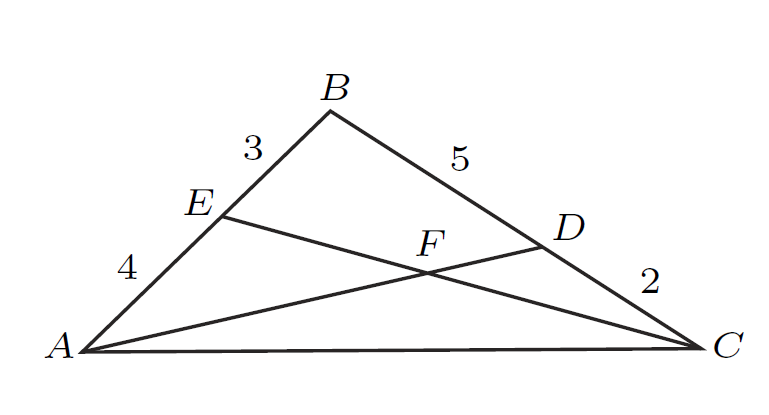
\includegraphics[width=2.5in]{cevian}
	\end{center}
\end{problem}
\begin{problem}
Point $E$ is selected on side $AB$ of $\triangle ABC$ in such a way that $AE : EB = 1 : 3$ and point $D$ is selected on side $BC$ so that $CD : DB = 1 : 2$. The point of intersection of $AD$ and $CE$ is $F$. Find $\frac{EF}{FC}+\frac{AF}{FC}$.
\end{problem}
\begin{problem}
In $\triangle ABC$ points $D$ and $E$ lie on $BC$ and $AC$, respectively. If $AD$ and $BE$ intersect at $T$ so that $AT/DT=3$ and $BT/ET=4$, what is $CD/BD$? (AMC)
\end{problem}

\subsubsection{Split Masses}
When we have a \textbf{transversal}, mass points are no longer intuitive. We have to use a method called \textit{split masses}, which help us approximate and eventually find out the answer. 

One way to think about the intuition behind split masses is to consider this: imagine that at the split mass point, let's call it $P$, it was actually two $P_1$ and $P_2$ that are \textit{very} close together. Now we can balance the two points like we normally do, and when we take the limit of the distance between $P_1,P_2$ to be zero, then the mass at $P$ will just be the sum of the component masses.
\begin{problem}
    In the figure below, $ED$ joins points $E$ and $D$ on the sides of $\triangle ABC$ forming a transversal. Cevian $BG$ divides $AC$ in a ratio of 3 to 7 and intersects the transversal $ED$ at point $F$. Find the ratios $EF : FD$ and $BF : FG$.
    \begin{center}
	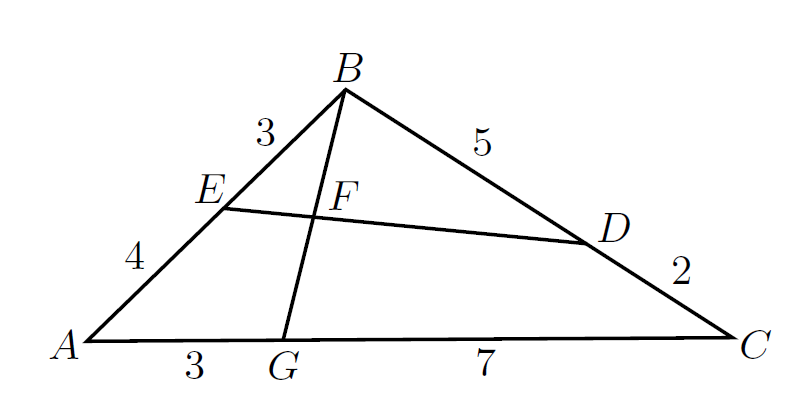
\includegraphics[width=2.5in]{transversal}
	\end{center}
\end{problem}
\begin{problem}
In $\triangle ABC$, point $D$ lies on $\overline{AB}$ such that $\overline{AD}=5$ and $\overline{DB}=2$, and point $E$ lies on $\overline{AC}$ such that $\overline{AE}=3$ and $\overline{EC}=8$. $F$ is the point of intersection of $\overline{BC}$ and the angle bisector of $\angle BAC$, and $G$ is the point of intersection of $\overline{AF}$ and transversal $\overline{DE}$. Find the ratio $AG:GF$. (TJ ARML Practice)
\end{problem}
\subsubsection{Systems}
\begin{problem}
In triangle ABC, points $D$ and $E$ are on sides $BC$ and $CA$, respectively, and points $F$ and $G$ are on side $AB$ with $G$ between $F$ and $B$. $BE$ intersects $CF$ at point $O_1$ and $BE$ intersects $DG$ at point $O_2$. If $FG = 1$, $AE = AF = DB = DC = 2$, and $BG = CE = 3$, compute $\tfrac{O_1O_2}{BE}$.
\end{problem}
\begin{problem}
In a triangle, segments are drawn from one vertex to the trisection points of the opposite side . A median drawn from a second vertex is divided, by these segments, in the continued ratio $x : y : z$. If $x \leq y \leq z$ then find $x : y : z$. (NYSML)
\end{problem}
\subsubsection{Get Creative}
\begin{problem}
In parallelogram $ABCD$, point $M$ is on $\overline{AB}$ so that $\frac {AM}{AB} = \frac {17}{1000}$ and point $N$ is on $\overline{AD}$ so that $\frac {AN}{AD} = \frac {17}{2009}$. Let $P$ be the point of intersection of $\overline{AC}$ and $\overline{MN}$. Find $\frac {AC}{AP}$. (AIME 2009 \#4)
\end{problem}
\begin{problem}
Triangle $ABC$ has $AB=21$, $AC=22$ and $BC=20$. Points $D$ and $E$ are located on $\overline{AB}$ and $\overline{AC}$, respectively, such that $\overline{DE}$ is parallel to $\overline{BC}$ and contains the center of the inscribed circle of triangle $ABC$. Then $DE=m/n$, where $m$ and $n$ are relatively prime positive integers. Find $m+n$. (AIME 2001 \#7)
\end{problem}
\begin{problem}
In triangle $ABC^{}_{}$, $A'$, $B'$, and $C'$ are on the sides $BC$, $AC^{}_{}$, and $AB^{}_{}$, respectively. Given that $AA'$, $BB'$, and $CC'$ are concurrent at the point $O^{}_{}$, and that $\frac{AO^{}_{}}{OA'}+\frac{BO}{OB'}+\frac{CO}{OC'}=92$, find $\frac{AO}{OA'}\cdot \frac{BO}{OB'}\cdot \frac{CO}{OC'}$. (AIME 1992 \#14)
\end{problem}